\chapter{Analyseklassendiagramm}
In Abbildung ~\ref{fig:akd} sind alle im Lastenheft erkannten Entitäten erfasst und es stellt die Beziehungen zwischen diesen umfassend dar. Diese Darstellungen sind durch die Analyse der Anwendungsfälle der Eventplanungssoftware sowie die Analyse des Lastenheftes entstanden.

\begin{figure}[ht!]
    \centering
    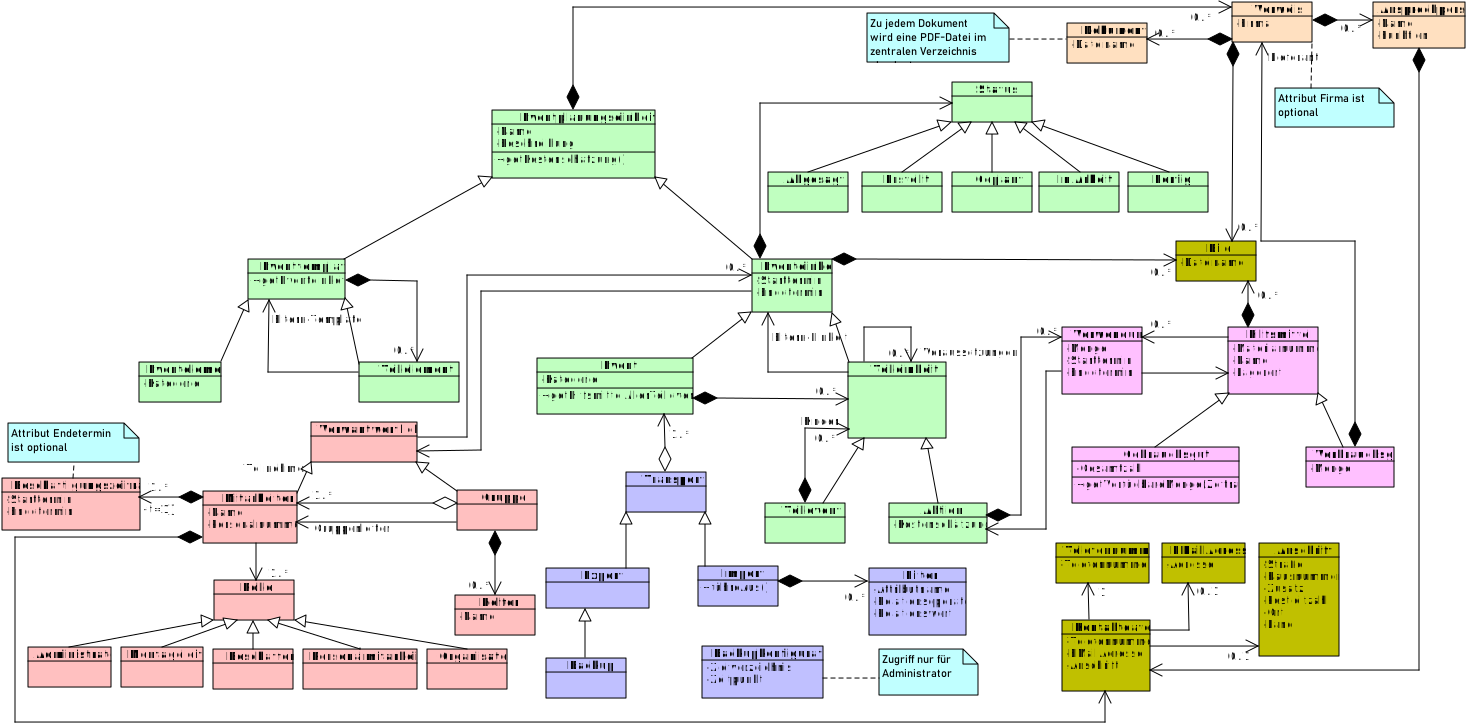
\includegraphics[width=0.98\columnwidth]{Bilder/akd.pdf}
    \caption{Analyseklassendiagramm mit Ansicht aller Objekte in der Eventplanung}
    \label{fig:akd}
\end{figure}

Zur Übersichtlichkeit wurden die Entitäten je nach Bereich eingefärbt. Alle dem Personal und der Verantwortlichkeit für eine Eventeinheit zuzuordnenden Entitäten sind rot eingefärbt, alle für Hilfsmittel wichtigen Klassen sind pink, alle das Transportsystem betreffenden Klassen sind violett. Die Klassen, welche die Struktur des Eventablaufes und dessen Planung betrachten sind grün eingefärbt, während Verweise und dazugehörendes orange sind. Alle Hilfsklassen, die zwischen zwei Bereichen stehen, sind grünbraun eingefärbt. Im Folgenden werden zuerst die einzelnen Entitäten erläutert und anschließend wird näher auf die verwendeten Analysemuster eingegangen.

\section{Analyse der verschiedenen Objekte}

\paragraph{Transport}
Ein Transportobjekt ist eine Aggregation von Events. Ein Transportobjekt sollte nie instantiiert werden, sondern nur die Unterklassen. Es beschreibt eine Menge an Events, die importiert, exportiert oder zur Datensicherung gespeichert werden sollen.
\paragraph{Export}
Exporte beschreiben eine Menge an Events im System, die exportiert werden sollen. Der Export findet zur Datensicherung im Falle eines Backups statt und sonst zur Weitergabe bestimmter Eventdaten. Die Events für den Export werden anhand von Filtern ausgewählt und dann in dem Exportobjekt gesammelt.
\paragraph{Import}
Ein Importobjekt ist eine aus einer Datei gelesene Ansammlung von Events, die dafür bestimmt sind, in das System hinzugefügt zu werden. Auf diesen Import können Filter angewendet werden, bevor dieser mit \code{führeAus()} die dann noch durch die Filter ausgewählten Events im System einpflegt.
\paragraph{Filter}
Ein Filterobjekt wird dafür verwendet, eine Teilmenge von Events aus einer Obermenge auszuwählen. Dafür werden jeweils der Name des Attributs gespeichert, mit dem verglichen werden soll, der Vergleichsoperator, der dafür verwendet werden soll und der Wert, mit dem verglichen werden soll. Damit können jegliche simple Filter realisiert werden, wie zum Beispiel, dass der Starttermin später als 2020 ist. Diese Filter können beispielsweise bei Export- und Import-Aktionen verwendet werden.
\paragraph{Backup}
Ein Backup ist eine spezielle Form des Exports, bei dem alle Events zur Datensicherung auf einem externen Medium gespeichert werden. Backups können automatisch wöchentlich durch die Backupkonfiguration festgelegt stattfinden oder manuell von einem Administrator ausgeführt werden.
\paragraph{Backupkonfiguration}
Die Backupkonfiguration legt zentral fest, wann wöchentliche Backups stattzufinden haben und in welchem Zielverzeichnis diese abgelegt werden sollen. Die Backupkonfiguration kann von einem Administrator verändert werden.

\paragraph{Verweis}
Ein Verweisobjekt ist eine zentrale Zusammenfassung aller Daten zu einem externen Objekt, häufig einer Firma. Er enthält ein einziges Attribut zum Festhalten des Firmennamens, welches optional ist, damit auch nicht-Firmen-Verweise dargestellt werden können. Ein Verweis enthält eine Sammlung an Dokumenten, Bildern und Ansprechpersonen. Diese Objekte sind jeweils nur vorhanden, solange auch der Verweis existiert. Sie werden also gelöscht, wenn der Verweis gelöscht wird. Ein Verweis muss kein weiteres Objekt enthalten, sondern kann auch vollkommen leer initialisiert werden. Der Hauptnutzen eines Verweises ist es, externe Dokumente und Objekte im System abzubilden, damit sie vom Nutzer eingesehen werden können.
\paragraph{Dokument}
Das Dokumentobjekt beschreibt ein von einem Nutzer zu einem Verweis hinzugefügtes Dokument, welches er für zukünftige Zwecke festhalten möchte. Dabei wird als Attribut der Dateiname gespeichert, den die Datei im zentralen Verzeichnis hat, auf dem Dokumente und Bilder abgelegt werden. Dokumente können nur einem Verweis hinzugefügt werden, jedoch nicht einem Event direkt. Beispielhaft für ein Dokument wäre ein Mietvertrag, der einem Verweis auf die verwendete Halle einer Hochzeit zugeordnet wird.
\paragraph{Ansprechperson}
Das Ansprechpersonobjekt beschreibt eine Kontaktperson zu einem Verweis. Dieses ist zum Beispiel der Hausmeister einer Halle oder der Verkäufer bei einem Lieferanten. Dafür werden der volle Name sowie die Funktionsbezeichnung dieser Kontaktperson gespeichert. Der Name wird als einzelnes Attribut gespeichert, damit jegliche Kombination von Name, Vorname und Mittelnamen vollständig und ohne Probleme abgebildet werden kann, ohne dass jede Besonderheit einzeln im Modell beachtet werden muss. Zu der Kontaktperson werden auch noch Kontaktdaten gespeichert, damit gesichert ist, dass diese immer kontaktiert werden kann.

\paragraph{Verantwortlicher}
Eine Eventeinheit benötigt immer exakt einen Verantwortlichen, der die Verantwortung dafür trägt, dass diese Eventeinheit erfolgreich und vollständig abgeschlossen wird. Diese Verantwortung kann von einer Einzelperson oder einer Gruppe mit Gruppenleiter getragen werden. Damit ist immer eine Einzelperson identifizierbar, die dafür verantwortlich ist, aber auch abgebildet, dass mehrere Personen an der Erfüllung der Aufgabe beteiligt sein können.
\paragraph{Gruppe}
Ein Gruppenobjekt beschreibt, dass eine Menge an Menschen an dem Teilevent oder Event arbeitet. Jede Gruppe hat exakt einen Gruppenleiter, der gleichzeitig auch ein Teilnehmer der Gruppe ist, daher hat jede Gruppe mindestens einen Teilnehmer. Die Teilnehmer einer Gruppe sind Mitarbeiter des Unternehmens. Des Weiteren kann eine Gruppe noch Helfer beinhalten, die auch an der Eventeinheit beteiligt sind.
\paragraph{Helfer}
Ein Helferobjekt stellt einen Helfer dar, der nicht bei dem Unternehmen angestellt ist. Zu diesen Helfern wird nur der Name gespeichert. Dadurch ist es möglich, schnell und einfach externe Hilfskräfte im System festzuhalten. Da sich externe Hilfskräfte in der Vergangenheit als äußerst unzuverlässig erwiesen haben, wird sich in der Planung nicht auf deren Anwesenheit verlassen. Externe Hilfskräfte sind zum Beispiel die Mutter der Braut, die gerne dabei helfen möchte, die Stühle aufzubauen. Dafür wird sie im System als Helfer eingetragen, sodass der verantwortliche Gruppenleiter darüber Bescheid weiß.
\paragraph{Mitarbeiter}
Über jeden Mitarbeiter werden im System Daten zu Name, Personalnummer, den Berechtigungen, Kontaktdaten und Beschäftigungszeiträumen gespeichert. Es müssen nicht viele Daten über diesen gespeichert werden, da der Großteil bereits im Personalbuchhaltungssystem verwaltet wird und für die Eventplanung nicht notwendig ist. Jeder Mitarbeiter kann befristet oder unbefristet eingestellt sein. Zur Zeit nicht eingestellte Mitarbeiter werden weiter im System behalten, um so zum Beispiel Saisonarbeiter verwalten zu können, die immer wieder ein befristetes Verhältnis mit dem Unternehmen eingehen.
\paragraph{Beschäftigungszeitraum}
Im Beschäftigungszeitraumobjekt werden jeweils der Starttermin und der Endetermin eines Beschäftigungsverhältnisses zwischen einem Mitarbeiter und dem Unternehmen festgehalten. Dieses ist wichtig, um planen zu können, ob befristete Mitarbeiter bei einem zukünftigen Event noch zur Verfügung stehen oder bereits nicht mehr eingestellt sind. Dadurch sind auch Saisonarbeiter gut unterstützt, die nur während der Hochsaison für Events eingestellt werden.
\paragraph{Rolle}
Die Rollen eines Mitarbeiters beschreiben seine Berechtigungen im System. Jeder Mitarbeiter hat mindestens eine Rolle und kann jede Rolle höchstens einmal haben. 
\begin{itemize}
    \item \textbf{Administrator} - Die Administratorrolle gibt dem Mitarbeiter die Berechtigung alles zu tun, was eine andere Rolle kann und noch die Backups zu konfigurieren und auszuführen. Diese Rolle ist nur zum Aufsetzen und für administrative Zwecke im System erforderlich.
    \item \textbf{Montageleiter} - Der Montageleiter hat das Recht, ihm zugewiesene Teilevents im Kontext zu sehen, um die ihm damit zugewiesenen Aufgaben erledigen zu können.
    \item \textbf{Beschaffer} - Der Beschaffer hat das Recht, ihm zugewiesene Teilevents im Kontext zu sehen, um die ihm damit zugewiesenen Aufgaben erledigen zu können. Des Weiteren kann dieser Hilfsmittel verwalten.
    \item \textbf{Personalmitarbeiter} - Personalmitarbeiter sind für die Verwaltung des Personals zuständig. Sie können Mitarbeiter verwalten, ihnen Rollen zuweisen oder ihre Beschäftigung verändern. Sie sind auch dafür verantwortlich, relevante Daten aus dem Personalbuchhaltungsprogramm in dem Eventplanungssystem festzuhalten.
    \item \textbf{Organisator} - Der Organisator plant Events, daher kann er Eventplanungseinheiten verwalten. Dazu zählt es, diese anzulegen, zu bearbeiten oder auch zu löschen. Des Weiteren kann der Organisator Events importieren und exportieren.
\end{itemize}

\paragraph{Status}
Die Klasse Status bildet die Oberklasse aller Status, in welchen sich eine Eventeinheit, also ein Event oder Teilevent befinden kann. Damit besitzt der Status die folgenden Unterklassen, welche jeweils einen konkreten Status repräsentieren:
\begin{itemize}
    \item \textbf{Erstellt} - In diesem Status befindet sich eine Eventeinheit unmittelbar nach dem Anlegen und während der Planungsaktivitäten.
    \item \textbf{Geplant} - Ist die Planung einer Eventeinheit sowie ihrer untergeordneten Teilevents vollständig abgeschlossen, so befindet sich die Eventeinheit im Status \enquote{Geplant}.
    \item \textbf{In Arbeit} - Während der eigentlichen Durchführung einer Eventeinheit befindet sich diese im Status \enquote{In Arbeit}.
    \item \textbf{Fertig} - Ist eine Eventeinheit vollständig abgeschlossen, so befindet sie sich im Status \enquote{Fertig}. 
    \item \textbf{Abgesagt} - Ist eine Eventeinheit nicht mehr durchzuführen, so wird diese in den Status \enquote{Abgesagt} gesetzt.
\end{itemize}

\paragraph{Bild}
Da einer Vielzahl von Objekten auch Bilder zugeordnet werden können, bedarf es für diese auch eine programmatische Repräsentation. Dies geschieht mittels der Klasse Bild, welche jedoch als Attribut lediglich den Namen der zugehörigen Bilddatei besitzt, anhand welchem das Bild geladen werden kann, sobald notwendig.

\paragraph{Verwendung}
Die Klasse Verwendung bildet die Zuweisung von Hilfsmitteln zu Aktionen ab. Hilfsmittel werden durch eine Verwendung jeweils in einer bestimmten Menge über einen bestimmten Zeitraum gebucht. Darum besitzt die Verwendung als Attribute die Menge sowie einen Start- und einen Endetermin. Sie verweist außerdem jeweils auf das gebuchte Hilfsmittel sowie auf das Teilevent, für welches das Hilfsmittel gebucht wird.

\paragraph{Kontaktdaten}
Da sowohl zu Ansprechpersonen als auch zu Mitarbeitern Kontaktdaten gespeichert werden müssen, werden diese durch eine separate Klasse abgebildet. Diese besitzt Assoziationen zu Telefonnummer, EMailAdresse und Anschrift. Allerdings sind EMailAdresse und Anschrift optional, lediglich eine Telefonnummer ist verpflichtend.

\paragraph{Eventplanungseinheit}
Die Eventplanungseinheit ist die Oberklasse der nachfolgend beschriebenen Klassen Eventtemplate und Eventeinheit. Sie liefert die primitiven Attribute Name und Beschreibung sowie eine Getter-Methode für die Kostenschätzung der jeweiligen Einheit. Hierbei haben Instanzen der Eventplanungseinheit ohne weitere Untereinheiten (Unterteilevents oder Unterteilelemente) eine manuell einzutragende Kostenschätzung, bei allen anderen ist die Kostenschätzung die Summe der Kosten der Untereinheiten. Ferner besitzt jede Eventplanungseinheit beliebig viele Verweise.

\paragraph{Eventemplate}
Das Eventtemplate bildet wiederum die Oberklasse des Eventelements und des Teilelements, da es sich bei beiden um vorgefertigte Templates für Eventeinheiten, also Events bzw. Teileinheiten handelt. Jedes Eventtemplate besitzt beliebig viele untergeordnete Teilelemente. Es handelt sich hierbei um eine Komposition, da die Existenz der untergeordneten Teilelemente von der des Eventtemplates abhängt. Ferner besitzt das Eventtemplate die Methode \code{getEventeinheit()}, welche aus dem Template ein Eventelement bzw. ein Teilelement mit voreingestellten Attributwerten generiert.

\paragraph{Eventelement}
Bei dem Eventelement handelt es sich um ein Template für ein Event. Es besitzt außer den von den Überklasssen Eventplanungseinheit und Eventtemplate geerbten Attributen noch das Attribut Kategorie. Dieses ermöglicht es, dem Event ein Schlagwort wie \enquote{Hochzeit} oder \enquote{Kongress} zuzuordnen.

\paragraph{Teilelement}
Bei einem Teilelement handelt es sich um ein Template für eine Teileinheit. Es besitzt ebenfalls die Attribute der Oberklassen Eventplanungseinheit und Eventtemplate. Darüber hinaus besteht eine Assoziation zu seinem Eltern-Template. Hierbei kann es sich entweder um ein weiteres Teilelement oder ein Eventelement handeln.

\paragraph{Eventeinheit}
Die zweite Unterklasse der Eventplanungseinheit ist die Eventeinheit. Sie wiederum bildet die Oberklasse des Events sowie der Teileinheit und liefert die Attribute Starttermin und Endetermin. Beide Attribute beinhalten jeweils ein Datum und eine minutengenaue Uhrzeit. Ferner besitzt jede Eventeinheit stets einen Status. Bei dieser Assoziation handelt es sich um eine Komposition, da ein einzelner Status ohne zugehöriges Objekt keinen Sinn ergeben würde. Des weiteren können jeder Eventeinheit beliebig viele Bilder zugewiesen werden. Da die Bilder mit einer Eventeinheit fest verknüpft sind und nicht unabhängig von diesen existieren können, handelt es sich auch bei dieser Assoziation um eine Komposition.

\paragraph{Event}
Die Klasse Event erbt von der Oberklasse Eventeinheit. Sie erweitert diese um das Attribut \enquote{Kategorie}, welches analog zum gleichnamigen Attribut des Eventelements die Möglichkeit bietet, dem Event ein bestimmtes Schlagwort zuzuordnen. Ein Event hat beliebig viele untergeordnete Teileinheiten, welche nur gekoppelt mit dem Event existieren können. Daher ist diese Assoziation als Komposition modelliert worden. Da das Event keine eigenen Hilfsmittel besitzt, sondern lediglich die Hilfsmittel der ihm untergeordneten Teilevents kumuliert, besitzt es die Methode \code{getHilfsmittelAllerEvents()}, welche eine Liste aller den untergeordneten Teileinheiten zugewiesenen Hilfsmitteln liefert.

\paragraph{Teileinheit}
Ebenso wie das Event erbt auch die Teileinheit von der Oberklasse Eventeinheit und ist selbst Oberklasse von Teilevent und Aktion. Da jede Teileinheit einer weiteren Teileinheit oder einem Event untergeordnet ist, besitzt es eine Assoziation zu einer Eventeinheit, nämlich die ihm übergeordnete Elterneinheit. Ferner können einzelne Teileinheiten von anderen Teileinheiten abhängig sein. So müssen beispielsweise vor dem Aufbau der Tischdekoration bei einer Hochzeit erst die Tische aufgebaut werden. Um derartige Umstände abzubilden, besitzt jede Teileinheit beliebig viele Voraussetzungen, also Teileinheiten, welche zuvor abgeschlossen sein müssen.

\paragraph{Teilevent}
Das Teilevent stellt eine Menge an Teileinheiten dar, die inhaltlich zusammen gehören und somit zusammen geplant werden. Es erbt von der Teileinheit und hat beliebig viele Teileinheiten als Kinder.

\paragraph{Aktion}
Eine Aktion ist eine konkrete Tätigkeit, die durchgeführt wird und nicht weiter in kleinere Tätigkeiten zu zerteilen ist. Daher hat diese Aktion dann auch eine konkrete, manuell eingetragene Kostenschätzung und der Aktion können Hilfsmittel zugeordnet werden. Um dieses zu tun, verweist diese auf beliebig viele Verwendungen, die jeweils die Buchung eines bestimmten Hilfsmittels darstellen. Folglich werden diese beim Löschen eines Teilevents ebenfalls gelöscht, daher handelt es sich bei dieser Assoziation um eine Komposition.

\paragraph{Hilfsmittel}
Für die meisten Events werden Hilfsmittel benötigt. Dies können beispielsweise Tische und Stühle, Kerzen auf einer Hochzeit oder ein Rednerpult für einen Kongress sein. Jedes Hilfsmittel besitzt als Attribute eine eindeutige Materialnummer sowie einen Namen und einen Lagerort. Ferner verweist jedes Hilfsmittel auf beliebig viele Verwendungen, welche die Buchung eines Hilfsmittels für einen bestimmten Zeitraum in einer bestimmten Menge darstellen. Es werden allerdings zwei verschiedene Arten von Hilfsmitteln unterschieden, welche über die beiden Unterklassen Gebrauchsgut und Verbrauchsgut der Klasse Hilfsmittel unterschieden werden. 

\paragraph{Gebrauchsgut}
Die Klasse Gebrauchsgut erbt von der Klasse Hilfsmittel und repräsentiert Hilfsmittel, welche mehrmals verwendet werden und der Abnutzung unterliegen. Zu jedem Gebrauchsgut wird die vorhandene Gesamtzahl gespeichert, außerdem besitzt es die Methode \code{getVerfügbareMenge()}, welche die in einem gegebenen Zeitraum verfügbare Menge des Hilfsmittels bestimmt.

\paragraph{Verbrauchsgut}
Die Klasse Verbrauchsgut erbt ebenfalls von der Klasse Hilfsmittel und repräsentiert Hilfsmittel, welche nur einmal verwendet werden können, wie beispielsweise Kerzen. Da diese direkt nach der Buchung als verbraucht gelten, ist für die Verbrauchsgüter keine besondere Methode zur Mengenberechnung nötig, sondern es wird lediglich die derzeit verfügbare Menge gespeichert. Da diese Hilfsmittel außerdem regelmäßig nachbestellt werden müssen, verweist jedes Verbrauchsgut auf einen Lieferanten.

\section{Verwendete Analysemuster}
Es wurden verschiedene Analysemuster verwendet, um die Objekte der Analyse zu modellieren. Analysemuster sind schematische Lösungen für eine Klasse verwandter Probleme. Es wurden die nachfolgenden fünf Analysemuster im Analyseklassendiagramm verwendet.
\paragraph{Rollen}
Das Analysemuster der Rollen wurde bei der Assoziation von Gruppe auf Mitarbeiter verwendet, um den Gruppenleiter von restlichen Teilnehmern zu differenzieren. Ein Mitarbeiter, der Teilnehmer einer Gruppe ist, kann zugleich der Gruppenleiter einer anderen oder der gleichen Gruppe sein. Daher ist es sinnvoll diese Unterscheidung durch Rollen vorzunehmen.

\paragraph{Koordinator}
Bei der Verwendung wurde das Analysemuster des Koordinators angewendet, um zu speichern, in welchem Zeitraum und welcher Menge ein Hilfsmittel bei der Aktion verwendet wird. Damit beinhaltet die Verwendung Attribute, die für die Beziehung zwischen den Objekten wichtig sind, aber in keinem der Objekte richtig aufgehoben wären.

\paragraph{Historie}
Mit der Klasse Beschäftigungszeitraum wurde das Analysemuster Historie verwendet. Die einem Mitarbeiter zugeordneten Instanzen dieser Klasse bilden den zeitlichen Verlauf seines Anstellungsverhältnisses bei der Firma ab. Durch die Attribute \enquote{Starttermin} und \enquote{Endetermin} ist für jede Instanz der Zeitraum festgelegt. Zwar ist hierbei der Endetermin optional, dies ist jedoch notwendig, um unbefristete Beschäftigungsverhältnisse abzubilden. In diesem Fall ist der Endetermin implizit noch nicht eingetroffen oder geplant.   

\paragraph{Liste}
Das Analysemuster Liste wurde im vorliegenden Analyseklassendiagramm an zwei Stellen verwendet. Im folgenden werden diese genauer erläutert.
\begin{itemize}
    \item Jedes Event beinhaltet eine Liste von ihm untergeordneter Teileinheiten. Die Teileinheiten eines Events sind diesem fest zugeordnet und können nicht ohne es existieren, lassen sich aber löschen ohne dabei das gesamte Event zu löschen. Abweichend von der Norm kann das Event jedoch auch keine Teileinheit beinhalten, also leer sein.
    \item Analog zum Event beinhaltet das Eventtemplate eine Liste von ihm untergeordneten Teilelementen. Auch diese sind dem Eventtemplate fest zugeordnet und können nicht ohne sie existieren, lassen sich aber löschen ohne dabei das gesamte Eventtemplate zu löschen. Allerdings kann auch das Eventtemplate keine Teileinheit enthalten und weicht in dieser Hinsicht leicht von der Norm ab.
\end{itemize}

\paragraph{Stückliste}
Das Analysemuster der Stückliste wurde bei der Aufteilung der Teileinheit in Teilevent und Aktion als Ganzes und Teil in einer Baumstruktur verwendet. Dadurch können die Bedürfnisse des Kunden optimal abgebildet werden, da einer Aktion eine Kostenschätzung und Hilfsmittel zugeordnet werden, dem Teilevent als Menge mehrerer Teileinheiten jedoch nicht direkt. Hier ist nur ein Typ an Blättern, die Aktionen, vorhanden.